\section{Introduction}

Every day, more and more people and objects connect, communicate and transfer data with each other. In today's world, we need both speed and security for our communications, even if both were considered two opposite ends of a spectrum. By adding error correction and encryption to our data, we can increase reliability and privacy at the expense of latency.

Modern technologies, like the Internet of Things (IOT) and the Cooperative Autonomous Driving (CAV), are becoming more and more popular and necessary in our society. But they are highly demanding advancements, needing real-time communication and defense against dangerous disruptions.

We interact all the time with smart devices, capable of coordinating with each other in real time to reach a common goal. Multiple applications exist in wildfire prevention \cite{RAMADAN2024101248}, logistics \cite{Lee18042018}, home control \cite{9928254} and many more fields. These devices include sensors, cameras, agents, controllers and robotics. An important advantage we gain from these intricate, deeply connected networks is high efficiency and low error and incident rates.

With a declining population \cite{af1cfa15} that gets more productive by the day \cite{The-Productivity-Pay-Gap}, we are moving towards a future where technology can help us in a lot of mundane, repetitive and sometimes dangerous tasks, allowing people to express more freely their potential and contribute more to the well-being and advancement of humankind. Imagine a world where the house is cleaned automatically, the electricity bill is reduced by automatic control based on necessities, and autonomous driving vehicles move you wherever needed while you work on your most important objectives \cite{The-Promises-of-Automation}. This is a promising future, but there are a lot of obstacles to overcome first.

The load on our infrastructure grows faster than ever. Every day, more people and devices alike connect to the internet or with each other, sending and receiving even more data \cite{Cloudflare-Radar-2024-Year-in-Review}. Cable communications cost too much in terms of space and maintenance, and wireless communication challenges increase as the number of connected machines multiply. But at the same time, we need reliability and speed.

With our lives dependent on technology, we also need way more security. We cannot risk attacks from malicious users, because of the damage they may cause. Appliances may be hacked to spy or short-circuited \cite{Inside-the-Smart-Home-IoT-Device-Threats-and-Attack-Scenarios}, cars could be deceived and cause fatal crashes \cite{CAV-attack}. Critical infrastructure like hospitals are breached every day, exposing sensitive and crucial data to all malicious actors there could be \cite{Cyberattacks-in-healthcare}.

But at the same time, the rate of progress forbids us to choose between fast but unsecure communications, or encrypted and slow to capture ones. We need new ways, new paradigms to ensure safe data transfer with low latency and high accuracy.

Reconfigurable Intelligent Surfaces (RIS) are a new proposal that may help in this context. They are a low-power, low-cost solution to transform reflection from passive noise in our communications into active parameters we can fine-tune to redirect, expand and propagate our communication signals into more complex scenarios, for example by helping in situations without direct Line of Sight (LOS) \cite{SEGATA2024110443}.

RISs may help us expand our networks significantly, reaching more users, ensuring more speed and helping us with the reliability of the received signals.

In this thesis, we aid the research by expanding current literature and studying how to use RIS not only for the aforementioned reason, but also to protect our communication privacy against malicious eavesdroppers. We can modulate the reflection signal to make sure only the legitimate receivers can understand the message, while making the reflected signal be undecipherable and act as artificial noise to protect against unwanted listeners.

This is called Physical Layer Security (PLS): our objective is supporting higher levels of security, like encryption, to protect ourselves against adversary actors even when they have bigger resources than us, or reduce the complexity of it by ensuring less probability of capturing the signal in the first place \cite{5751298}.

Our plan is to serve as many users as needed, in complex scenarios without clear direct path between all the actors, while making the exchanged data unreadable for unwanted users. With our proposal, the signal is not undecipherable for anyone else, but it is completely unreadable from the start.

Imagine that instead of sending to everyone random letters, where only the legitimate receivers can understand what is written, we can also make sure that all the other unwanted listeners get not random letters, but random strikes. Even if they had unlimited resources and computational power, for example quantum computers, they would not be able to do anything because they have nothing to work on.

By adding this extra layer of security, we can then reduce the encryption power on the higher levels of communications, making messages faster to parse and understand. In critical high-speed communication like CAV, having a bigger throughput with lower latency can be critical in expanding the possible speed of every car in the network from scientific interest to usable, everyday technology.

\subsection{Our contribution}

The specific contributions of this work are:
\begin{itemize}
  \item a general explanation of the current advancements in Physical Layer Security and Reconfigurable Intelligent Surfaces
  \item a detailed explanation of a proposed signal modulation, called Space Shift Keying (SSK), and a proposed framework for RIS-aided encryption made by prominent researchers in the field
  \item generalize the framework to support multiple legitimate users, multiple RIS in series, and multiple signal paths in parallel, while keeping the same level of security and complexity
  \item carry out Bit Error Rate (BER) simulation analysis to prove the efficacy of our proposed solution
  \item model a realistic communication system to include channel gain matrix calculations, Rician fading and path loss
  \item in particular, study different configurations of path losses to give a better general vision of the applicability of our solution
  \item heatmap graphs to show the behavior in various practical scenarios
\end{itemize}

We will provide detailed mathematical explanation and extensive simulation code to better help the research in more future application studies about the application in real-life communications between physical actors.

\subsection{Notation}

We will use the following notations in this work:

% Variables, vectors, and matrices are written as italic letters \textit{x}, bold italic letters \textbf{x}, and bold capital italic letters \textbf{X}, respectively. For any vector x, diag{x} denotes a diagonal square matrix whose diagonal consists of the elements of x; dim{x} denotes the dimension of the vector. For any square matrix X, [X]diag denotes a diagonal square matrix formed by the diagonal elements of X. The operators E, Ex , Tr[·], (·)T , (·)† , (·)−1 , ∥·∥, and ∥·∥∞ denote the expectation with respect to all the randomness, the expectation with respect to x, the trace, the transpose, the Hermitian, the inverse, the Frobenius norm, and the infinity norm of their arguments, respectively. ⊙ is the Hadamard product. p(A) denotes the probability of the event A. Define IN = {1,2,...,N} as a shorthand as the index set. Ik and 0k denote the k-by-k identity and zero matrices, respectively. The default base of the logarithm is 2.

\begin{itemize}
  \item Variables are written as capital italic letters $X$
  \item Vectors are written as italic letters $x$
  \item Matrices are written as bold capital italic letters $\bm{X}$
  \item $\C$ defines the Complex set, $C^X$ a complex vector of length $X$, and $C^{X \times Y}$ a complex matrix of dimension $X$ rows and $Y$ columns
  \item given $x \in \C^Y$, we define $\bm{X} = diag\{p\} \in \C^{Y \times Y}$ a matrix with all zeros, except in the diagonal where position $y,y$ is equal to $x_y$
  \item given $\bm{X} \in \C^{Y \times Y}$, we define $x = diag(\bm{X}) \in C^Y$ the vector of the elements in the diagonal of $\bm{X}$
  \item given $\bm{X} \in \C^{Y \times Y}$, we define $\bm{X}_{diag} \in \C^{Y \times Y}$ the matrix with all zeros, except in the diagonal where position $y,y$ is equal to $\bm{X}_{y,y}$
  \item given $\bm{X} \in \C^{Y \times Z}$, we define $[\bm{X}]_{:,1:Y} \in \C^{Y \times Y}$ the first $Y$ columns of $\bm{X}$
  \item $\odot$ is the Hadamard product
  \item A Hermitian transpose of $\bm{V}$ ($\bm{V}^H$), means we first transpose the matrix ($\bm{V} \rightarrow \bm{V}^T$), then take the conjugate of every element (so invert the sign of the imaginary part).
  \item The Frobenius norm of a matrix $\bm{X}$, denoted as $\|\bm{X}\|$, is defined as $\|\bm{X}\| = \sqrt{\sum_{i}\sum_{j} |x_{ij}|^2}$
\end{itemize}

\newpage
\section{Related works}
\subsection{Physical Layer Security}

\textit{The essential premise of physical layer security is to enable the exchange of confidential messages over a wireless medium in the presence of unauthorized eavesdroppers, without relying on higher-layer encryption.}\cite{6739367}

Physical layer security is much lighter than complex secret key-based cryptographic techniques \cite{10599431}. It ensures high reliability and security at less computational cost. Being much quicker than the higher layer counterparts, it ensures low latency in higher bands, like 5G or 6G. Ultra-reliable low latency communication (URLLC) may help critical infrastructure in delivering high privacy and data speed capabilities. The ability to combine both lower and higher layer security will also enhance the general capabilities of everyday applications.

We have two types of threats we need to protect against. Active attacks, like jamming a frequency, disrupt and block the flow of information; while passive attacks, like eavesdropping, are more subtle and we need to make our signals undecipherable with encryption or noise \cite{5751298}. In particular, passive hearing could expose sensitive data, and even encryption may still leak location, traffic load and other sensitive information.

Modern communication needs multiple requirements in order to guarantee the efficacy and security of communications:
\begin{itemize}
  \item legitimate users should be authenticated
  \item access control must be implemented to ensure confidentiality of the messages
  \item integrity of the communication, to ensure the message is correctly delivered
  \item availability of the channel link, to ensure jamming attacks do not influence negatively the flow of information
  \item defense and encryption against eavesdroppers
\end{itemize}

There are different methods we can use to mask our communications: we can fingerprint the legitimate users, as explained in the paper \cite{228fe14543ce4cefba3bb9cc11741362}, use directional antennas to reduce the area where it is possible to capture the signal \cite{4543070}, or add artificial noise schemes to disrupt unwanted hearers \cite{1605889}.

Different error correction strategies can also mitigate the effect of active attacks. We can use some of the passed bits to ensure the data received is correct, and sometimes even fix the errors. We can also use \textit{Spread Spectrum Coding} to rapidly change the frequency used to deliver the message, ensuring difficulties in disrupting all of the available ones.

%%%%%%%%%%

Modeling the threats of adversaries can be quite challenging \cite{7120011}. Many research papers include assumptions that we need to be careful about. For example, eavesdroppers may not just be passive listeners, but may actually collect data to later transform into active attackers.

The adversaries may also have better resources, both in computer power and signal reception, and it is difficult to model all possible threats we may face. We may have multiple stations collaborating together in deciphering the signal, or even be backed up by national agencies. Some work has already been done addressing these issues: in \cite{5707054}, the authors study a universal coding scheme to protect against eavesdroppers changing constantly channels. In \cite{7543509} a statistical model is created to calculate the probability of achieving secrecy from eavesdroppers in unknown locations.

%%%%%%%%%

Achieving perfect communication secrecy is not really possible for all cases, given that we need the secret key to be at least as big as the secret message \cite{6769090}, but there are some practical strategies we can implement.

In particular to eavesdropping, there is a huge opportunity for improvements. While disruptions have been studied for long, especially in military communications, message encryption is usually delegated to the higher levels \cite{6739367}. However, the physical layer can assist by hiding or masking the signal, making it harder for the eavesdropper to capture it. Given the advances in quantum computing and encryption breaking algorithms \cite{365700}, it is important to be protected at all layers.

\subsection{Reconfigurable Intelligent Surface}

\begin{figure}[H]
  \centering
  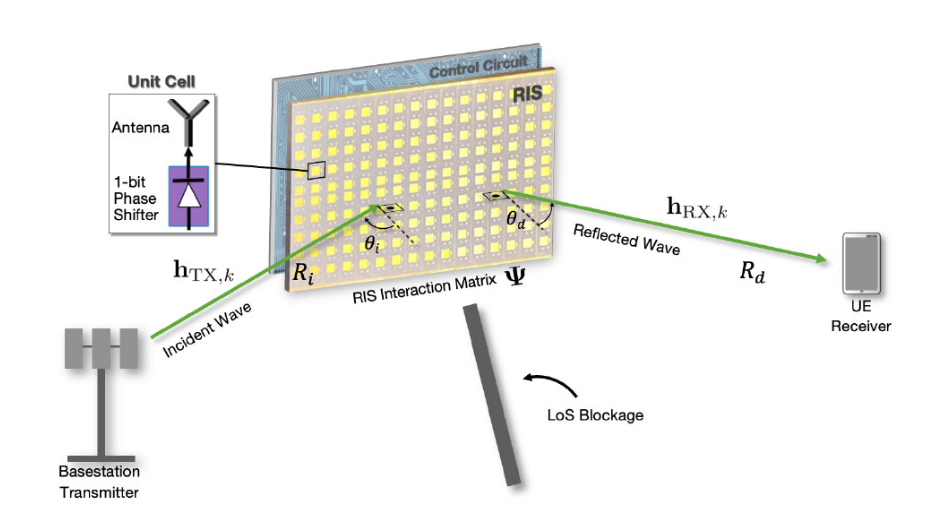
\includegraphics[width=0.5\linewidth]{imgs/RIS model.png}
  \caption{An example of possible design of a Reconfigurable Intelligent Surface [From \cite{9732917}]}
\end{figure}

Reconfigurable Intelligent Surfaces (RISs) are a new technology that can help in improving the security and reach of wireless communications. They are made of a large number of passive elements that can reflect the signals in a way that can be controlled and optimized.

With RISs, it is possible to control the propagation and reflection of radio waves, making it possible to transform the environment, in which the waves need to travel, from an uncontrollable phenomenon to a programmable variable that is possible to (partially) control and optimize.

RISs can help in particular in two scenarios. In the first one, two nodes which are not in the line of sight (LOS) can communicate with the help of the RIS; in the second one, being in the LOS means an inability to take advantage of delayed reflections (especially for new technologies like 5G and 6G), which can be used to improve the signal quality and robustness, but we can create them with RISs \cite{9086766}.

\begin{figure}[H]
  \centering
  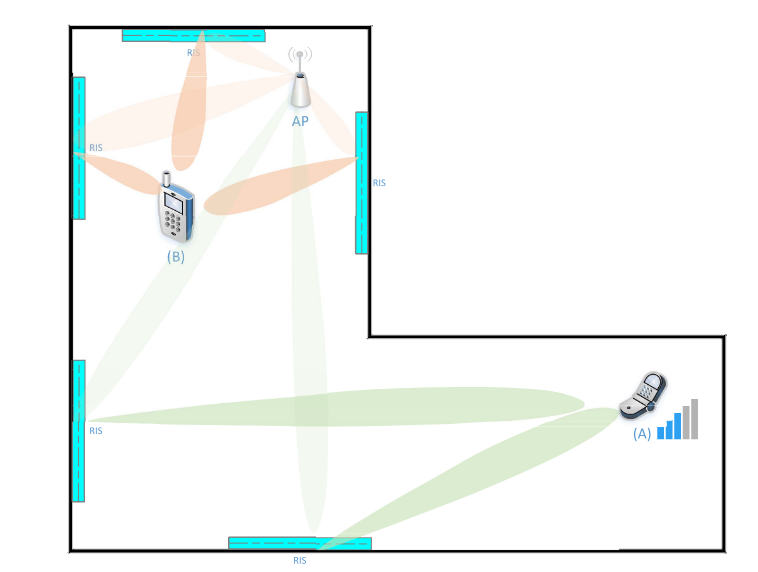
\includegraphics[width=0.5\linewidth]{imgs/RIS enviroment.png}
  \caption{\textit{A smart radio environment with multiple RISs. User A is far away
      from the AP and suffers from low received signal strength, while user B has
      ample received power but a low-rank ill-conditioned channel. The RISs can
      be optimized to help in both scenarios.} [From \cite{9086766}]}
\end{figure}

The main advantages of RISs are the low cost, the low power consumption and the easy deployment, which makes them a good candidate for the future of wireless communications. They do not require a dedicated energy source, they do not suffer from noise amplification, they can work with any frequency and can be easily put on any surface like walls or ceilings \cite{8796365}.

A specific controller is used to modify dynamically the reflecting elements of the RIS, giving huge margins for custom configurations in complex scenarios and new communications frameworks.

Numerous applications are being studied to this day. For example, in \cite{9881509} the authors study the modeling of path loss for a reflected signal; they then recreate a RIS using an Arduino to validate the mathematical calculations.

RIS can also be included in more general smart cities projects \cite{9253607}: in a more interconnected world, they can be used for everyday streets and personal homes; huge, unused building surfaces may aid the general population in getting better connectivity; smart factories and the industry 4.0 could be assisted in dense IoT device places, by countering the negative effects of metals for signal strength.

Active RIS can also be deployed \cite{9377648}, which can amplify the received signal before reflecting it, ensuring an even higher power output and reach for a similar design. Beamforming can also be used to redirect the signal towards a specific direction, increasing the signal strength for the receiver in that specific area.

\subsection{Using RISs for Physical Layer Security}

RISs can be used to greatly increase not only the network performance but also its security \cite{10409564}. By using RISs, we can make the signal quality better, reduce the signal degradation and make the signal more difficult to intercept by eavesdroppers.

For example, the reflection can be used as multiplicative randomness to make the transmission not understandable from eavesdroppers, while having a decoding for the legitimate user linear \cite{9328149}.

There is the possibility for attackers to also use RIS as an assistance tool to spy on communications, and even propagate jamming attacks in multiple directions \cite{10143983}.

\begin{figure}[H]
  \centering
  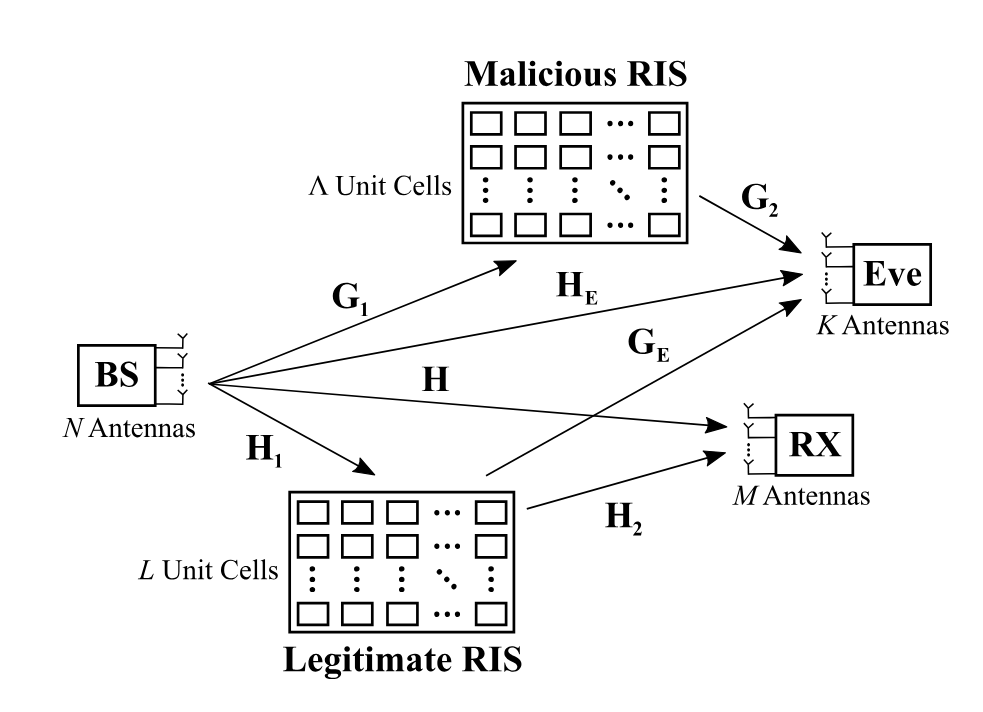
\includegraphics[width=0.5\linewidth]{imgs/RIS malicious.png}
  \caption{Eavesdroppers could not only listen from the transmitter or the legitimate RIS, but even deploy a malicious one, possibility for passive and active attacks [From \cite{10143983}]}
\end{figure}

Another paper \cite{s21041439} studied how to use a novel RIS based channel randomization technique to improve the secrecy rate, and another one \cite{8742603} shows an iterative efficient algorithm to maximize the minimum secrecy rate by optimizing the reflecting coefficients of the RIS.

RISs can also be used to protect against jamming attacks: for example, in \cite{9424472} an aerial RIS is used to mitigate the effects of the disturbance and increase the transmission power and reliability.

\subsection{RISs and Physical Layer Security for Vehicular Networks}

\begin{figure}[H]
  \centering
  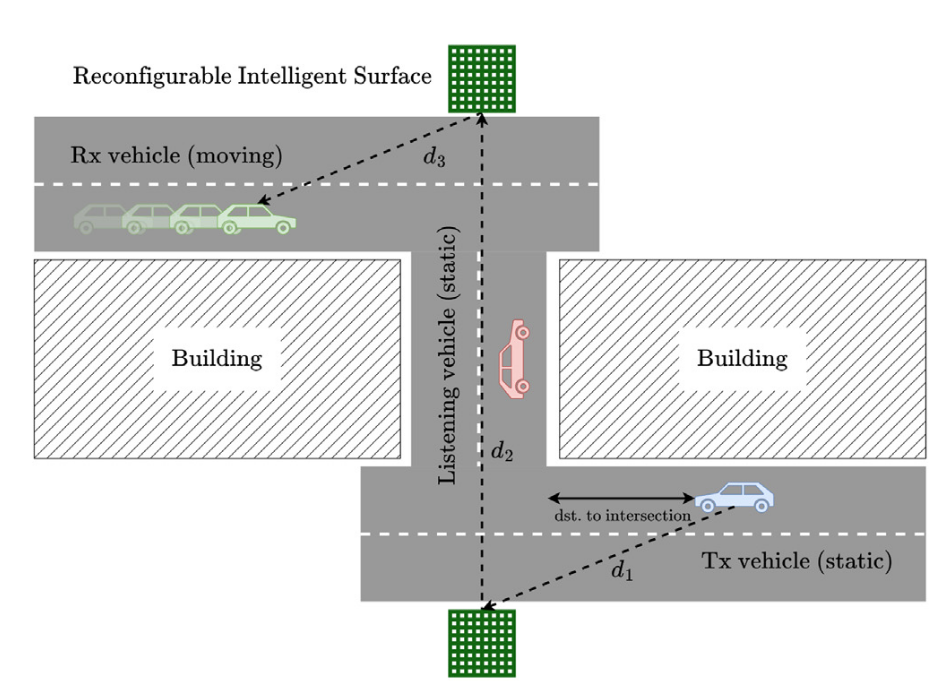
\includegraphics[width=0.5\linewidth]{imgs/RIS vehicles.png}
  \caption{An example of usage of RIS for vehicle communications [From \cite{SEGATA2024110443}]}
\end{figure}

Cooperative autonomous driving can bring many benefits, like reducing traffic congestion, improving road safety and reducing the environmental impact of the vehicles. Cars and other vehicles can communicate with each other and with the infrastructure to share information and coordinate their movements. However, it also brings new security concerns, especially in the wireless communications.

It is clear that it is necessary to have a secure and fast way to communicate, and 6G network technologies plus RISs can help in this regard. By reflecting the signals, we can overcome the limitations of LOS and improve the signal quality by reducing signal degradation \cite{10715713}.

The sector is just starting to be studied, but there are already some promising results. Network simulators made specific, like CoopeRIS, allow to study and progress in this field \cite{SEGATA2024110443}.

Vehicular networks need low latency and high security. Active attacks may jeopardize drivers' and people's safety, while also slowing down the information exchange rate. Being moving agents, it is more difficult to correctly model this type of network, but also way more necessary: complex upper layer encryption may slow down data processing enough to render it useless \cite{8403278}.

Passive attackers may instead use vehicles' geolocation and traffic data for malicious activity. A way to detect and filter out intruders is discussed in \cite{8474336}.

Recent studies show how RISs can be used to protect the vehicular network against illegitimate users. In \cite{makarfi2020reconfigurableintelligentsurfacesenabledvehicular} the authors study how RISs can improve the average secrecy capacity and secrecy outage probability.